\chapter{Digital filter}

\section{Design}

The goal of this lab is to digitally filter a waveform sampled at 44.1kHz and downsample it to a frequency of $F_{sampling}=22.05$ kHz. To perform this subsampling, it is necessary that the signal is composed of frequencies smaller than the Nyquist frequency : 
\[ F \le F_N = \frac{F_{sampling}}{2} \] 
Thus, all frequencies higher than $ F_N = 11.025$ kHz have to be filtered out by a low pass filter.\\
\\
As it is known, an ideal low pass filter is defined by its impulsional response: 
\[ h(n) = B*sinc(Bn) = B * \frac{sin(\pi*B*n)}{\pi*B*n} \] where \[B = 2*f_{cut}\]

\section{Evaluation}

\subsection{Theory}

The design is first evaluated in MATLAB, to check if the chosen architecture meets the task requirements. For this evaluation, the testbench consists of a sum of identical sinus waveforms of frequencies equally distributed between 0 and 20kHz, with a step of 1kHz. The resulting spectrums are given on figure \ref{fig:filterMatlabTestbench}. For the simulation, the order of the filter is fixed to 150.

\begin{figure}[!h]%
	\centering
	\subfloat[Original signal]{{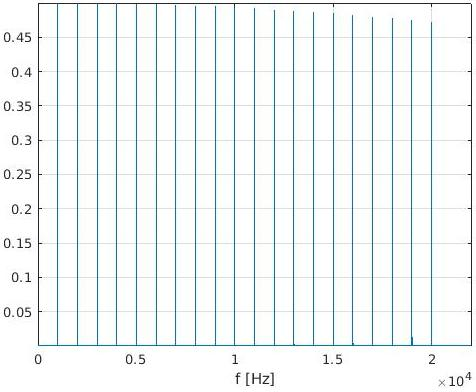
\includegraphics[scale=0.6]{images/Filter/input.jpg}}}%
	\qquad
	\subfloat[Filtered signal]{{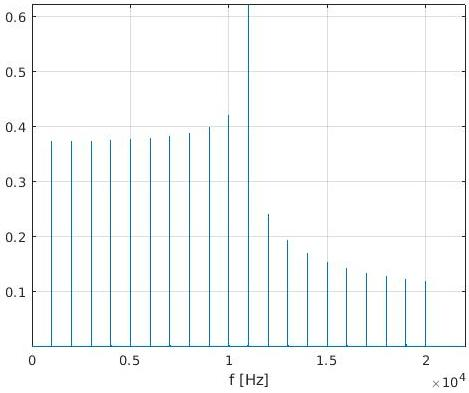
\includegraphics[scale=0.6]{images/Filter/response.jpg}}}%
	\caption{Spectrum (in magnitude) of the original and filtered signals}%
	\label{fig:filterMatlabTestbench}%
\end{figure}

As expected, the chosen filter has a low pass behavior with a cut frequency $F_c = 11.025 kHz$.

\subsection{Filter evaluation}

To evaluate the performance of the digital filter implemented in Verilog, a simulation is performed in Cadence. The testbench used for this purpose is to be found in \texttt{digital\_filter\_Testbench2}, and the corresponding schematic is provided in figure \ref{fig:filterTestbench}. it consists of a sum of sinus waveforms of 500Hz and 20 kHz respectively. For this simulation, an ideal ADC \texttt{adc\_ideal} has been additionally implemented, to convert the analog input signal to a digital one before filtering. The values for the different parameters are given in the table \ref{table:filterTestbench}. The order of the filter is deliberately small, in order to prevent a too important delay.\\
The obtained transient waveforms and spectrums are provided respectively in figures \ref{fig:filterCadenceTestbenchTransient} and \ref{fig:filterCadenceTestbenchSpectrum}.
 

\begin{figure}[!h]
	\centering 
	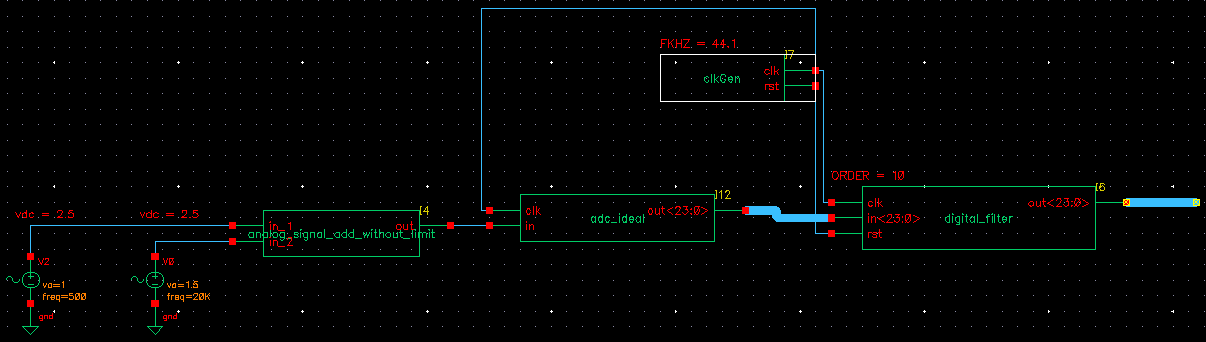
\includegraphics[scale=0.55]{images/Filter/testbench.png}
	\caption{Digital filter testbench}
	\label{fig:filterTestbench}
\end{figure} 

\begin{table}[!h]
	\centering
	\begin{tabular}{|l|r|}
		\hline
		Clock frequency (\texttt{FKHZ}) & 44.1 kHz \\
		\hline
		Filter order (\texttt{ORDER}) & 10 \\
		\hline
	\end{tabular}
	\caption{Filter testbench parameters}
	\label{table:filterTestbench}
\end{table}

\begin{figure}[!h]
	\centering 
	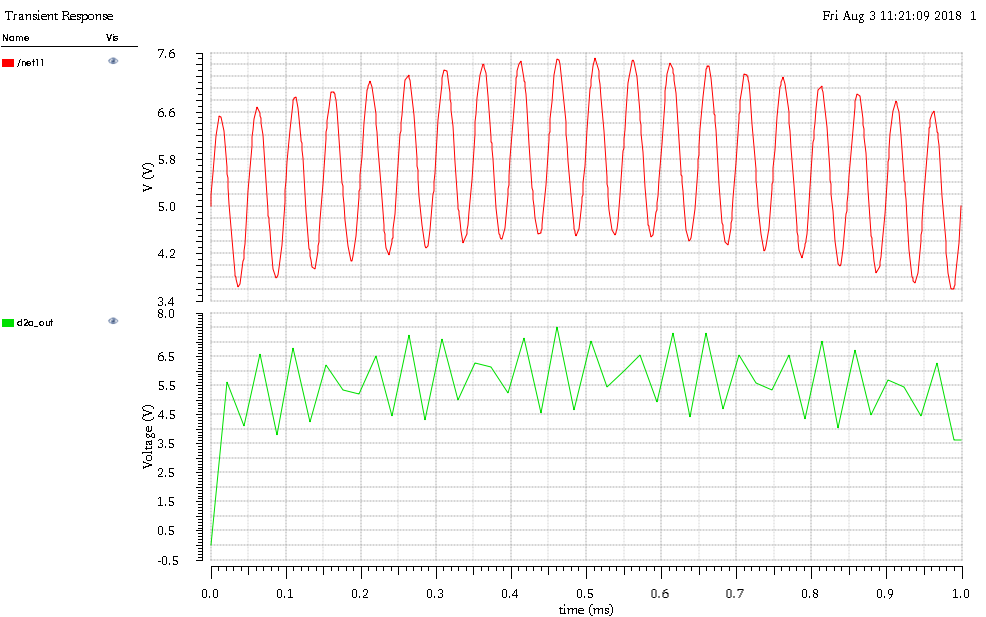
\includegraphics[scale=0.6]{images/Filter/signal.png}
	\caption{Transient simulation of the input (red) and filtered (green) signals}
	\label{fig:filterCadenceTestbenchTransient}
\end{figure} 

\begin{figure}[!h]
	\centering 
	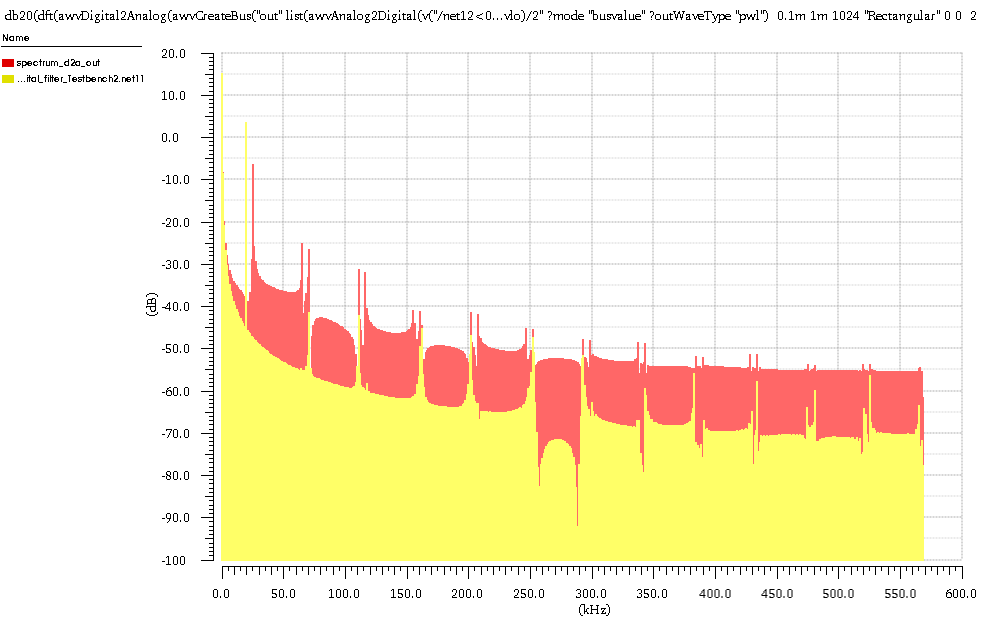
\includegraphics[scale=0.6]{images/Filter/spectrum.png}
	\caption{Spectrum of the input (yellow) and filtered (red) signals}
	\label{fig:filterCadenceTestbenchSpectrum}
\end{figure} 

Surprisingly, the filtered signal contains more noise as the input signal. This may be due to the ADC which is working only at 44.1 kHz and may not capture the whole complexity of the input signal. Moreover, the relatively small order does not allow the filter to have a sharp cut of the higher frequencies.

\section{Synthesis}

The synthesis of the digital filter described above is performed using Synopsis Design Vision. The statistics obtained for different clock period are given in the table \ref{table:synthesisStats}.

\begin{table}[!h]
	\centering
	\begin{tabular}{|r|r|r|r|r|}
		\hline
		 \multirow{2}{*}{\textbf{Frequency}}
		 & \multirow{2}{*}{\textbf{Clock period [ns]}}
		 & \multirow{2}{*}{\textbf{Slack [ns]}} & \multicolumn{2}{c|}{\textbf{Area}} \\
		 \cline{4-5}
		 & & & \multicolumn{1}{c|}{\textbf{Cell}} & \multicolumn{1}{c|}{\textbf{Total}} \\
		\hline
		 1 GHz & 1 & - 1.78 & 31790.520257 & 54632.811374 \\
		 500 MHz & 2 & - 0.75 & 31881.240270 & 54705.954386 \\
		 \rowcolor{Blue}
		 333 MHz & 3 & 0.00 & 28362.240120 & 51198.672295 \\
		 250 MHz & 4 & 0.00 & 24488.640096 & 44641.649983 \\
		 200 MHz & 5 & 0.00 & 24275.520098 & 44453.918988 \\
		 \rowcolor{Green}
		 100 MHz & 10 & 0.00 & 23325.840074 & 41648.888715 \\
		 1 Hz & $10^{9}$ & ~$10^{9}$ & 23018.760042 & 47767.179669 \\
		\hline
	\end{tabular}
	\label{table:synthesisStats}
	\caption{Filter synthesis statistics}
\end{table} 

As shown in table \ref{table:synthesisStats}, the maximal clock frequency of the implemented filter is \textbf{333 MHz} (that is, a minimal clock period of \textbf{3 ns}). As expected, the required (cell and total) area is generally increasing with the frequency. Thus, the minimal total area is obtained for a frequency of \textbf{100 MHz}.
